\begin{spacing}{1.5}
  \begin{tightcenter}
    \section{3. Diseño y metodología}
    \mylinespacing
  \end{tightcenter}

  En este capítulo se describen los métodos utilizados para el diseño y desarrollo del servicio de computación, así como el plan para su implementación.

  \subsection{3.1 Resultados esperados}

  En la siguiente tabla se muestran los logros proyectados para cada uno de los objetivos específicos estipulados en el marco de la tesis.

  \begin{table}[h]
    \centering
    \begin{tabular}{p{7cm}|p{7cm}}
      \hline
      \textbf{Objetivos Específicos}                                 & \textbf{Producto(s) Esperados} \\
      \hline
      Identificar recursos disponibles y necesidades investigativas. &
      Documento expresando la arquitectura de los recursos y las necesidades a
      considerar.                                                                                     \\
      \hline
      Diseñar una solución que considere los requerimientos de los usuarios y
      aproveche las capacidades de los recursos computacionales mediante la
      implementación de un gestor de cola de tareas.                 & Documentación, scripts,
      programas y pruebas básicas de operación que simplifiquen o automaticen el
      mantenimiento y administración del gestor de cola de tareas.                                    \\
      \hline
      Llevar a cabo la instalación, documentación y puesta a punto de
      herramientas que apoyen los procesos de investigación y docencia en el área de
      matemáticas, facilitando el uso del servicio.                  & Documentación, scripts y
      programas que automaticen y faciliten la utilización del servicio para los
      estudiantes o profesores.                                                                       \\
      \hline
      Llevar a cabo pruebas de uso de la infraestructura y de las
      aplicaciones desplegadas en este trabajo.                      & Reporte de pruebas en donde se
      evidencie la correcta funcionalidad y la eficiencia de los                                      \\
      \hline
    \end{tabular}
    \caption{Resultados Esperados}
    \label{table:table2}
  \end{table}

  \subsection{3.2 Tecnologías y aprovechamiento de espacios}
  \label{chap:3.2}
  En esta sección se presentan las diversas especificaciones tecnológicas
  seleccionadas para el proyecto en cuestión.

  \subsubsection{3.2.1 Sistema operativo}
  El sistema operativo utilizado para la instalación de los equipos en este
  proyecto es Rocky Linux.

  \textbf{¿Qué es Rock Linux?}

  Rocky Linux es una distribución de Linux que se basa en el código fuente de
  Red Hat Enterprise Linux (RHEL), el cual se compila y se distribuye de forma
  gratuita y de código abierto. Rocky Linux está diseñado para ser compatible con
  el mismo software, herramientas y aplicaciones que RHEL, y ofrece una
  alternativa de código abierto para los usuarios que anteriormente utilizaban
  CentOS. Lo cual resulta en una herramienta poderosa por la gran cantidad de
  software disponible para los entornos RHEL.

  Este tipo de distribución tipo enterprise está diseñada para ofrecer
  estabilidad y confiabilidad en entornos de producción. La distribución incluye
  una variedad de herramientas y utilidades que facilitan la gestión y el
  mantenimiento de sistemas informáticos, incluyendo servidores y estaciones de
  trabajo. Además, Rocky Linux es compatible con paquetes de software de
  terceros. \cite{RL-1}

  \textbf{Rocky Linux 9}

  La versión específica del software utilizado es Rocky Linux 9 (*complete
  iso o DVD iso*) \cite{RL9-download-1} \cite{RL9-release-1}
  \cite{RHEL-release-1}

  Rocky Linux 9 ofrece soporte para actualizaciones de seguridad de este
  software hasta el 31 de Mayo de 2032 \cite{RL9-EOL-1}. Debido su estabilidad y
  largo ciclo de vida que ofrece, es ideal para minimizar las actualizaciones
  manuales a versiones mayores, lo que simplifica el mantenimiento requerido en
  el largo plazo.

  \textbf{Kernel}

  El kernel o núcleo es la parte central de un sistema operativo. Es el
  componente que se encarga de controlar el hardware y los recursos del sistema.
  El kernel es responsable de administrar la memoria del sistema, asignando y
  liberando recursos de manera eficiente. También se encarga de administrar los
  procesos y subprocesos del sistema, lo que permite que múltiples programas se
  ejecuten al mismo tiempo.

  El kernel es esencial para el funcionamiento del sistema operativo y
  proporciona una capa de abstracción entre el hardware y el software.
  \cite{RHEL-kernel-1}

  El kernel incluido en Rocky Linux 9 es la versión 5.14 LTS, que es bastante
  reciente. Esto significa que tanto los ordenadores antiguos, así como los más
  nuevos en la sala de cómputo pueden beneficiarse de esta actualización, y
  aquellos que se planeen comprar en el futuro cercano también podrán
  aprovecharla. \cite{RL9-release-1}

  \subsubsection{3.2.2 Sistema de Archivos}

  \textbf{XFS}

  Rocky Linux, al igual que RHEL utiliza por defecto XFS como sistema de
  archivos. XFS es un sistema de archivos de alto rendimiento que se utiliza en
  sistemas operativos Linux. Fue desarrollado por Silicon Graphics en la década
  de 1990 y se ha incorporado en el kernel de Linux desde la versión 2.4.

  XFS está diseñado para manejar grandes volúmenes de datos y archivos.
  Algunas de las características de XFS incluyen:

  \begin{itemize}
    \item Alta capacidad de lectura y escritura de archivos.
    \item Sistema de administración de archivos de registro que permite una
          recuperación rápida después de un fallo del sistema.
    \item Sistema de cuotas de disco para limitar el uso de espacio en
          disco por usuario o grupo.
  \end{itemize}

  XFS es una buena opción para sistemas que manejan grandes cantidades de
  datos y aplicaciones que requieren una alta capacidad de lectura y escritura de
  archivos. \cite{RHEL-XFS-1}

  \textbf{NFS}

  NFS (Network File System) es un protocolo de red de alto rendimiento y
  eficiente que permite a los sistemas informáticos compartir archivos y recursos
  a través de una red. Está diseñado para reducir la carga en la red y en el
  servidor. El protocolo utiliza una caché para reducir la cantidad de
  solicitudes de red y aumentar la velocidad de acceso a los recursos
  compartidos. Además, soporta la transferencia de datos en modo ráfaga, lo que
  permite que los datos se transfieran en grandes bloques en lugar de pequeños
  paquetes, lo que aumenta la eficiencia de la transferencia de datos. Es un
  estándar para compartir archivos en sistemas operativos basados en Unix y
  Linux.

  NFS se basa en el modelo cliente-servidor, donde un servidor exporta un
  sistema de archivos o un directorio a través de la red, y los clientes pueden
  montar este sistema de directorio en sus propios sistemas, lo que les permite
  acceder a los archivos y recursos compartidos como si estuvieran en su propia
  máquina.

  El protocolo NFS utiliza un sistema de autenticación y autorización para
  controlar el acceso a los recursos compartidos. Los clientes deben autenticarse
  con el servidor antes de acceder a los recursos compartidos, y el servidor
  puede configurar los permisos de acceso en base a las credenciales de los
  usuarios. \cite{RHEL-NFS-1} \cite{RHEL-NFS-2}

  \subsubsection{3.2.3 Distribución de Aplicaciones}
  Existen diversas opciones para la instalación de aplicaciones en Rocky
  Linux. Una de las formas más comunes es a través del uso de gestores de
  paquetes, como DNF, que permiten descargar e instalar software desde
  repositorios compatibles. Además, también es posible utilizar Flatpak, que
  ofrece una mayor flexibilidad en cuanto a la selección de versiones de
  aplicaciones y resolución de dependencias. Otra opción es mediante el uso de
  Podman, una alternativa más segura a Docker, aunque esta alternativa puede
  resultar más compleja y no es recomendada para usuarios inexpertos.

  En nuestro caso se planificó el uso de Flatpak con Flathub como medio
  principal para la instalación de aplicaciones, debido a que se ejecuta en un
  ambiente encapsulado, evitando así conflictos con las dependencias del sistema.
  Las aplicaciones o librerías que no se pueden obtener de Flathub se instalan
  mediante distintos repositorios.

  \textbf{Repositorios}

  Rocky Linux de base solo cuenta con sus propios repositorios de software,
  lo que acarrea un problema en la insuficiente variedad de programas y
  herramientas. Sin embargo, también existen otros repositorios compatibles
  populares como EPEL (Extra Packages for Enterprise Linux), que proporciona
  software adicional para sistemas basados en Red Hat Enterprise Linux, y RPM
  Fusion, que ofrece una gran cantidad de paquetes de software de código abierto
  que no están disponibles en los repositorios oficiales de la distribución. Al
  tener acceso a estos repositorios, se puede disfrutar de una selección de
  software y herramientas más completa. \cite{RL-repo-1} \cite{RHEL-EPEL-1}
  \cite{rpmfusion-1}

  \textbf{Flatpak}

  Flatpak es un sistema de paquetes de software que permite la distribución
  de aplicaciones de forma independiente de la distribución de Linux. Esto
  significa que los usuarios de Linux pueden descargar e instalar aplicaciones de
  una tienda centralizada (Flathub) sin preocuparse por las diferencias en la
  distribución de Linux que estén utilizando.

  Además, Flatpak se basa en contenedores, lo que significa que las
  aplicaciones y todas sus dependencias se empaquetan en un contenedor aislado.
  Esto permite a las aplicaciones ejecutarse de forma independiente de otras
  aplicaciones y bibliotecas del sistema, lo que ayuda a garantizar la
  estabilidad y la seguridad.

  También existe una tienda centralizada donde los usuarios pueden descargar
  e instalar aplicaciones. La tienda se llama Flathub, es un lugar con una amplia
  selección de software disponible sin costo alguno.

  La mayor ventaja de Flatpak y la razón por la que se escoge como método
  principal para instalar aplicaciones en el sistema es debido al aislamiento de
  dependencias, lo que evita conflictos con el sistema operativo. \cite{FLAT-1}
  \cite{FLAT-2} \cite{RHEL-FLAT-1} \cite{PHOENIX-FLAT-1}

  \textbf{Podman}

  Aunque se proveen las librerías y aplicaciones más comunes en la
  configuración que se realizó, con los distintos repositorios mencionados y el
  uso de flatpaks, hay usuarios que podrían tener aún más necesidades y más
  específicas, por lo que también se tiene Podman como soporte para usuarios
  avanzados.

  Podman es una herramienta de administración de contenedores para Linux.
  Permite a los usuarios crear, ejecutar y gestionar contenedores de manera
  similar a otras herramientas populares, como Docker. Sin embargo, a diferencia
  de Docker, Podman no requiere un servicio del sistema para ejecutar los
  contenedores, lo que significa que estos se ejecutan como procesos normales del
  usuario y pueden administrarse utilizando herramientas y comandos. Además,
  Podman utiliza el concepto de 'pods' en lugar de 'servicios', lo que permite a
  los usuarios agrupar y gestionar varios contenedores relacionados juntos en una
  única entidad lógica.

  Podman es una herramienta de código abierto y se desarrolla como parte del
  proyecto de código abierto de la comunidad de Red Hat. \cite{RHEL-podman-1}

  \subsubsection{3.2.4 Sala de cómputo Jürgen Tischer}

  La sala de cómputo es un lugar principalmente utilizado para impartir clases, pero también podría ser utilizada en los espacios libres para llevar a cabo tareas de cómputo distribuido. Es importante tener en cuenta que, debido a que la sala de cómputo es un espacio compartido, es necesario coordinar con los demás usuarios para evitar conflictos y asegurarse de que todos tengan acceso al equipo y los recursos necesarios.

  \textbf{Wolfram Mathematica}

  En el marco de este proyecto, se llevará a cabo una utilización efectiva de
  las licencias que actualmente se encuentran disponibles en la universidad. Se
  han identificado diversas herramientas y software matemáticos que son de gran
  utilidad para la realización de diversas tareas en el ámbito académico y
  científico, y la universidad cuenta con licencias para tres de ellas: Wolfram
  Mathematica, gridMathematica y MathLM.

  Estas licencias representan una valiosa oportunidad para la comunidad
  universitaria de utilizar herramientas de alta calidad y prestigio en el campo
  de las matemáticas, lo que permitirá mejorar el desarrollo de investigaciones,
  proyectos y actividades en general.

  Wolfram Mathematica es un sistema de software de álgebra computacional
  utilizado en matemáticas, física, ingeniería, ciencias sociales y otros campos.
  Ofrece una amplia gama de capacidades que incluyen análisis simbólico y
  numérico, visualización de datos, programación, modelado de sistemas y más.
  \cite{Wolfram-mathematica-1}

  MathLM es una herramienta de licencia de red de Mathematica que permite a
  las instituciones controlar y administrar el acceso de los usuarios al
  software. Con MathLM, las organizaciones pueden asignar licencias a usuarios
  individuales o grupos de usuarios, lo que les permite acceder al software desde
  cualquier lugar de la red. \cite{Wolfram-mathlm-1}

  gridMathematica es una herramienta de computación distribuida que permite a
  las instituciones y organizaciones compartir la carga de procesamiento de
  Mathematica en múltiples computadoras. Al distribuir el procesamiento de
  cálculos complejos en múltiples sistemas, gridMathematica puede reducir
  significativamente el tiempo necesario para realizar análisis complejos y
  simulaciones. También proporciona un mecanismo para administrar recursos
  computacionales y asegurar que las tareas se distribuyan de manera eficiente.
  Wolfram gridMathematica es una extensión de las capacidades de paralelización
  integradas de Mathematica que ejecuta más tareas en paralelo, en más CPUs y
  GPUs, para una ejecución más rápida. Automatiza la coordinación y gestión de
  procesos sin necesidad de cambios en el código. \cite{Wolfram-grid-1}

  \subsubsection{3.2.5 Clúster Bochica}

  El clúster Bochica es un espacio que cuenta con recursos informáticos, los cuales se planean aprovechar en el marco de esta tesis para llevar a cabo tareas de cómputo general y distribuido. Es importante destacar que, debido a su capacidad, este clúster podría permanecer activo para el uso remoto de usuarios de la universidad que soliciten acceso, siempre y cuando se coordinen las tareas y se respeten los recursos disponibles en el mismo.

  En el clúster Bochica, se planea aprovechar los recursos mediante la implementación conjunta de dos tecnologías: Slurm y JupyterHub. La combinación de estas dos herramientas permitirá a los usuarios del clúster ejecutar trabajos de cómputo de manera eficiente, al mismo tiempo que garantiza la seguridad y el control de acceso a los recursos.

  \textbf{SLURM}

  Como se ha mencionado anteriormente SLURM (acrónimo de Simple Linux Utility for Resource Management) es un sistema de gestión de recursos utilizado en entornos de computación de alto rendimiento (HPC). 
  
  \begin{figure}[h]
      \centering
      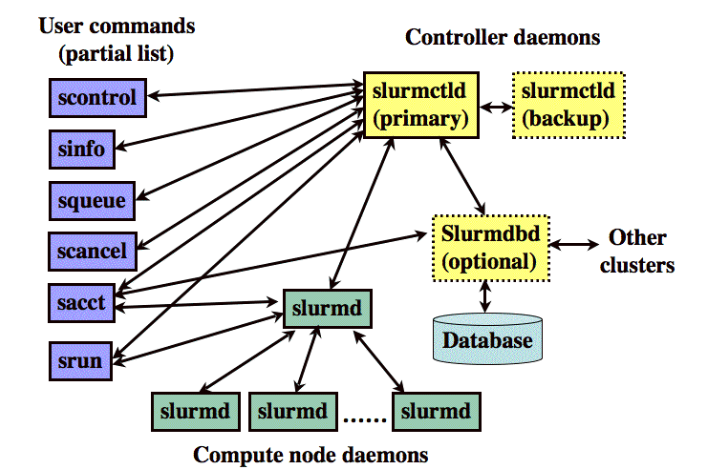
\includegraphics[width=0.8\textwidth]{slurm.png}
      \caption{Configuración SLURM}
      \label{fig:etiqueta}
    \end{figure}
  
  Algunas de las razones por las que se escoge Slurm para la gestión de recursos son:\cite{RHEL-SLURM-1}


  \begin{enumerate}
    \item Escalabilidad: Slurm es altamente escalable y puede manejar
          eficientemente grandes cargas de trabajo y múltiples usuarios en entornos de
          computación de alto rendimiento.
    \item Flexibilidad: Slurm es altamente configurable y permite a los
          usuarios definir y personalizar políticas de gestión de recursos, tales como
          prioridades de trabajos, particiones de clusters, políticas de colas, etc. Esto
          permite que Slurm se adapte a las necesidades específicas de cada grupo.
    \item Eficiencia: Slurm está diseñado para minimizar la sobrecarga del
          sistema y maximizar la eficiencia del uso de los recursos. Esto se logra
          mediante el uso de técnicas avanzadas de planificación y asignación de
          recursos, lo que garantiza que los trabajos se ejecuten de la manera más
          eficiente posible.
    \item Soporte de múltiples arquitecturas: Slurm soporta una amplia
          variedad de arquitecturas de hardware, incluyendo x86, ARM, IBM Power y otras
          arquitecturas de procesador.
    \item Comunidad activa: Slurm es un proyecto de código abierto con una
          comunidad de usuarios y desarrolladores activa y comprometida. Esto significa
          que hay una gran cantidad de recursos y soporte disponible en línea para ayudar
          a los usuarios de Slurm.
  \end{enumerate}

  Se anticipa que la implementación y utilización de Slurm resultará ser
  menos compleja que la de HTCondor, lo que confiere una mayor accesibilidad a la
  comunidad universitaria.

  \textbf{Jupyterhub}

  En el marco de este proyecto, se ha contemplado la utilización de JupyterHub como plataforma de acceso a los recursos computacionales, lo que permitirá a los usuarios disfrutar de una interfaz sencilla, centralizada y automatizada.

 JupyterHub es una plataforma sumamente versátil que se presta de manera excepcional para la gestión y ejecución simultánea de diversas instancias de Jupyter Notebook. Esta herramienta, por tanto, representa una alternativa idónea para contextos educativos o de investigación en los que varios usuarios necesitan emplear Jupyter Notebook de forma paralela.

  \begin{figure}[h]
      \centering
      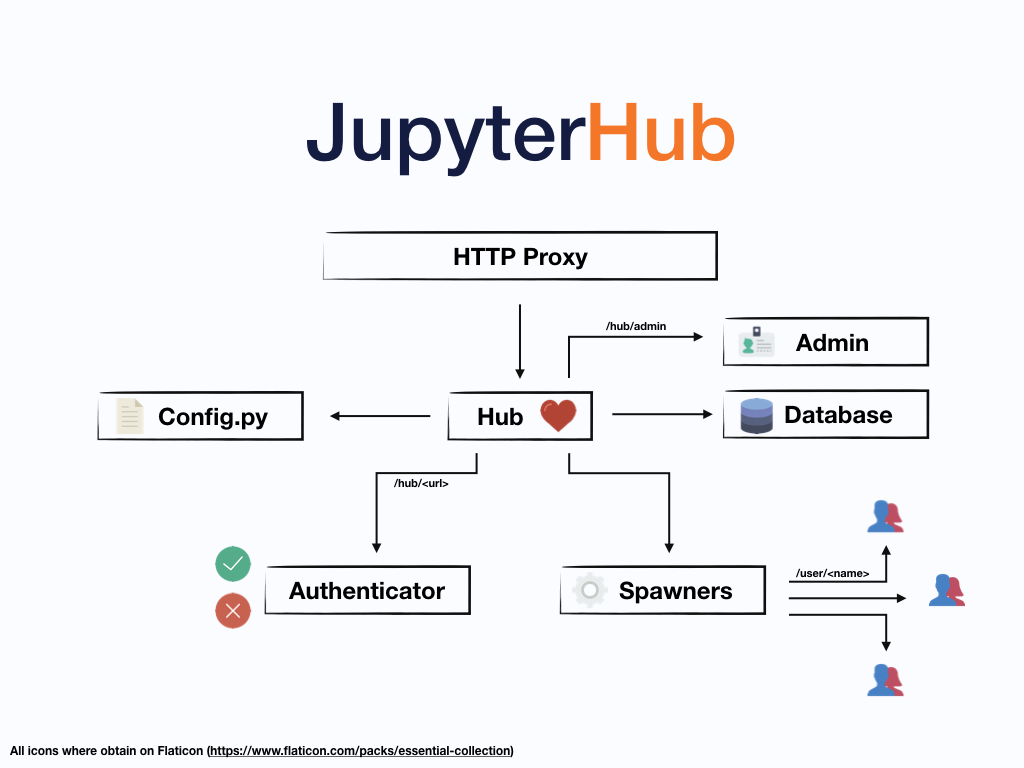
\includegraphics[width=0.7\textwidth]{hub.jpeg}
      \caption{Configuración JupyterHub}
      \label{fig:etiqueta}
    \end{figure}

    Al ejecutarse a través de un servidor central, el software de JupyterHub permite a los usuarios iniciar y detener sus sesiones de Jupyter Notebook de manera independiente. De esta manera, cada usuario dispone de su propio espacio de trabajo seguro y aislado en el que puede generar, llevar a cabo y compartir sus cuadernos de Jupyter, al tiempo que ofrece a los administradores de sistema un control riguroso del acceso y la seguridad de las múltiples instancias que se ejecutan.

    Con Slurm y JupyterHub, los usuarios del clúster podrán aprovechar al máximo los recursos disponibles y trabajar de manera más eficiente y colaborativa.

  \mylinespacing
  \mylinespacing
  \begin{tightcenter}
  \end{tightcenter}
\end{spacing}